%Anfoderungsanalyse

%%%%%%%%%%%%%%%%%%%%%%%%
\chapter{Analyse}
\label{sec:Anforderungsanalyse}
%%%%%%%%%%%%%%%%%%%%

\section{Informationsbedarf}
Der Informationsbedarf orientiert sich maßgeblich an den Aufgaben und dem Nutzer.

Was soll unterstützt werden?

\subsection{Modulare Anlage}
Der Lebenszyklus einer modulare Anlage wird in unterschiedliche Phasen eingeteilt. Sie besteht aus Planung, Errichtung, Betrieb und Demontage. \cite{} Besonderes Augenmerk in dieser Arbeit liegt auf dem Potential der Flexibilität. So kann die modularen Anlage beispielsweise bei Wartungsarbeiten an einem Modul mit einem alternativen Modul weiter betrieben werden.

Probleme können in modularen Anlagen auf verschiedenen Ebenen entstehen. Zum einen auf direkter Modulebene. So stellt das Modul beispielsweise entsprechende Alarme zur Verfügung. Dann können Probleme auch in Zusammenhang mit verschiedenen Modulen entstehen. Welche Probleme auftreten können ist in Abschnitt x näher beschrieben.

Um Probleme lösen zu können muss unter anderem klar sein, welche Informationen zur Verfügung stehen. Für den Austausch von Informationen zwischen Prozessführungsebene (PFE) und Modul wird das Modul Type Package (MTP) verwendet. Da der Modulhersteller entscheiden kann, welche Informationen zur Verfügung gestellt werden unterscheidet sich der konkrete Inhalt des MTP von Modul zu Modul. Es soll hier nicht auf den konkreten Aufbau des MTPs eingegangen werden.

\subsubsection{Informationsaustausch mittels MTP}
Das Modul stellt eine Reihe an Informationen zur Verfügung, die durch das Modul Type Package (MTP) beschrieben sind. Im MTP sind unter anderem das HMI und die Services hinterlegt.

Für einen eindeutigen Austausch von Informationen sind Schnittstellen definiert. Jede Schnittstellendefinition besteht aus einem Erklärungstext und den spezifischen Informationsvariablen. Da für jede Schnittstelle andere Informationen übertragen werden, sind hier nur allgemeine relevante Aspekte gelistet. So können Einheiten, Maximal- und Minimalwerte oder Prozesswerte übermittelt werden.
\begin{itemize}
\item \textbf{TagName:} Name der repräsentierten Information. 
\item \textbf{TagDescription:} Beschreibung der repräsentierten Information, z.B. Innere Temperatur des Reaktors.
\item \textbf{ScaleSettings:} Das Modul teilt der PFE die möglichen Anzeigegrenzen mit.
\item \textbf{UnitSettings:} Übermittelt die Einheit des übertragenen Werts.
\item \textbf{ValueLimitation:} Das Modul gibt die Sollwertgrenzen für bestimmt Parameter vor.
\item \textbf{Feedback Monitoring:} Gibt die Rückmeldung an die PFE, dass eine Fehlfunktion vorliegt.
\item \textbf{Limit Monitoring:} Mittels der Limit Variablen können Werte für Toleranz-, Warnungs- und Alarmgrenzen festgelegt werden. Das Modul überwacht die Variablen und signalisiert eine Grenzwertüberschreitung.
\end{itemize}

\subsubsection{Services}
Wie bereits in Abschnitt \ref{2:Modulare-Anlagen} beschrieben werden Module durch Dienste gesteuert. Jeder Dienst kann 16 verschiedene Zustände annehmen und teilt den aktuellen Zustand der PFE mit. Die PFE kann die Zustandsübergänge Reset, Pause, Resume, Unhold, Stop, Abort und Restart anfordern. Bei kontinuierlichen Fahrweisen können zusätzlich Start und Complete angefordert werden. Des weiteren wird der Zustandübergang State Change (SC) durch den vorgelagerten Zustand ausgelöst. \todo{Bild einfügen} Die aktuell verfügbaren Zustandswechsel meldet das Modul zurück.

Dienste haben verschiedene Betriebsarten. Sie werden in Offline, Manual, Automatic External und Automatic Internal eingeteilt. Zudem gehört zu jedem Dienst eine Liste mit dem verwendeten Anlagenequipment. Wenn sich der Dienst nicht in Offline befindet werden automatisch alle zum Dienst gehörigen Aktoren in Automatic überführt.
\begin{itemize}
\item \textbf{Offline:} Dienst ist nicht betriebsbereit und die Aktoren des Dienstes können in Manual überführt werden.
\item \textbf{Manual:} Der Dienst wird vom Bediener über die PFE oder ein lokales Panel bedient.
\item \textbf{Automatic External:} Die Zustandsübergänge werden durch die PFE gesteuert.
\item \textbf{Automatic Internal:} Die Zustandsübergänge werden modulintern ausgelöst.
\end{itemize}

Sollen Dienste näher spezifiziert werden, ist eine Verwendung von Parametern möglich. Es wird zwischen Konfigurationsparameter, Fahrweisenparametern, Prozesswerten und Reportwerten unterschieden.
\begin{itemize}
\item \textbf{Konfigurationsparameter:} Werden für grundlegende Einstellung verwendet. Ein Ändern ist nur möglich, wenn der Dienst offline ist. Es können beispielsweise ...
\item \textbf{Fahrweisenparameter:} Sind rezeptrelevant, werden vom Dienst beim Starten und Neustart überprüft und bei Zulässigkeit übernommen. Es wird an die PFE rückgemeldet, ob der Parameter übernommen werden konnte. Beispielhafte Parameter sind Sollwerte, wie Temperatur- oder Durchflussvorgaben und Reglerparameter, wie Verstärkung und Nachhaltezeit.
\item \textbf{Prozesswerte:} \todo{ergänzen}
\item \textbf{Reportwerte:} Zur Nachweis- und Dokumentationspflicht werden die Werte in den Zuständen Completed, Aborted und Stopped gespeichert.
\end{itemize}

\subsubsection{Probleme in modularen Anlagen}
Da die modularen Anlagen mit Diensten gesteuert werden ändern sich auch die Art an Problemen die entstehen und die vom Modulbetreiber behoben werden können. Durch die Dienste wird nur noch ein Problembereich angezeigt. Meldet ein Dienst zurück, dass er nicht erfolgreich durchgeführt werden kann so ist noch nicht eindeutig, wo das Problem liegt. Durch die Anzeige von dazugehörigem Equipment und möglichen Serviceabhängigkeiten kann der Problembereich eingegrenzt werden. Bei Betrieb der modularen Anlage treten derzeit die häufigsten Fehler auf, wenn entsprechende Zuläufe nicht geöffnet werden. So meldet aktuell das Modul nicht zurück, wenn vergessen wurde die Druckluft anzustellen. Dem Betreiber fällt nur auf, dass das Modul nicht so arbeitet, wie es soll. Wurde beim Temperiermodul vergessen den Zulauf für das Wasser zur Kühlung zu öffnen so meldet sich dieses erst nach ca. zwei Minuten zurück, dass es zu warm wird.

Insbesondere mit dem großen Vorteil der Flexibilität von modularen Anlagen können Probleme auch auf anderen Ebenen entstehen. Die Option nicht nur Parameter anzupassen sondern auch Module auszutauschen eröffnet neue Möglichkeiten und stellt den Modulbetreiber vor neue Herausforderungen. 

\subsection{Use Case}


\subsection{Informationen nach Aufgabenbereich}
Neben den Informationen, die ein Modul zur Verfügung stellt und die bei Behebung einer Störung behilflich sein können, gibt es eine Reihe von weiteren interessanten Aspekten. Weitet man den Problembereich von einer reinen Instandhaltung auf Bereiche wie die zunehmend geforderte Einsparung von Kosten aus, so werden ganz andere Informationen benötigt. Welche Funktionen auf welcher Ebene in einem Unternehmen automatisiert werden können und somit auch sinnvoll durch ein Assistenzsystem unterstützbar sind ist in \cite{Lauber1999} beschrieben. Hier ist auch der zeitliche Aspekt mit aufgeführt. Eine entsprechende Übersicht findet sich in Tabelle \ref{tab:Ebenen-Unternehmen}.
\begin{table}[htb]
\centering
\caption{Ebenen in einem Unternehmen bei Führung technischer Prozesse}
\label{tab:Ebenen-Unternehmen}
\begin{tabular}{|p{0.2 \textwidth}|p{0.33 \textwidth}|p{0.33 \textwidth}|}
\hline
\textbf{Ebenen eines Unternehmens} & \textbf{zeitliche Anforderungen} & \textbf{Automatisierungs-funktionen} \\
\hline
Unternehmens-führung & Entscheidungen wirken sich langfristig aus (nach Monaten oder Jahren) & Kostenanalysen, statistische Auswertungen \\
\hline
Produktions-planung und Betriebsleitung & Änderungen werden nach Tagen, Wochen oder Monaten sichtbar & Betriebsablaufplanung, Kapazitätsoptimierung, Auswertung der Prozessergebnisse \\
\hline
Leitung technische Prozesse & Eingriffe wirken sich nach Stunden oder Minuten aus & Prozessüberwachung, An- und Abfahrten, Störungsbehandlung, Prozessführung, Prozesssicherung \\
\hline
Prozessgrößen & Auswirkungen sind nach Sekunden, Millisekunden oder gar Mikrosekunden sichtbar & Messen, Steuern, Stellen, Regeln, Verriegelungen, Not-Bedienen von Prozessgrößen, Abschalten, Schutz \\
\hline
\end{tabular}
\end{table}

Auf der Unternehmensführungsebene sind beispielsweise folgende Kosten relevant \todo{eventuell löschen, da doppelt} \cite{Kunstler2014}:
\begin{itemize}
\item Logistikkosten
\item Personalkosten
\item Verpackungskosten
\item Kosten für Reklamationen und Retouren
\item Kosten aufgrund fehlender Prozesssynchronisation
\end{itemize}
Folgende Kennzahlen sind für die Produktions- und Betriebsleitebene interessant \cite{Kunstler2014}:
\begin{itemize}
\item \textbf{Kennzahlen der Beschaffung:} Lieferzeiten, Preistrends nach Warengruppen
\item \textbf{Kennzahlen der Produktion:} Auslastung der Geschäftsbereiche, Durchlaufzeiten, Rüstzeiten
\item \textbf{Kennzahlen der Finanzprozesse:} Produktivität- und Wirtschaftlichkeitskennzahlen
\end{itemize}

\subsection{Informationsbedarf der Operator}
Stützt man sich bei der Ermittlung des Informationsbedarfs auf die individuellen Fähigkeiten und das vorhandene Wissen so ist eine entsprechende Analyse relativ komplex. Insbesondere, wenn der Problemlöseprozess einen Lerneffekt haben soll. In der Literatur ist dies als Assistance Dilemma bezeichnet. Wenn der Lerneffekt möglichst groß sein soll wird Information über die Problemlösung und die Lösungsschritte zunächst zurück gehalten. Informationen werden interaktiv hinzugefügt, wenn sie benötigt werden. Die größte Herausforderung ist dabei die Kriterien festzulegen, wann Informationen gegeben und wann sie zurück gehalten werden. \cite{}  X empfiehlt eine geringe Bereitstellung an hilfreichen Erklärungen bei Problemlöseaktivitäten solange andere Ressourcen für den Lernprozess zur Verfügung stehen. Übertragen auf die Problemstellung dieser Arbeit lässt sich Schlussfolgern, dass alle relevanten Informationen zugänglich sein müssen. Diese sollten jedoch nicht alle direkt zu Beginn des Problemlöseprozess präsentiert werden. In Abschnitt x ist bereits beschrieben, dass komplexe Probleme auf das Wesentliche reduziert werden müssen und häufig Informationsbeschaffung gefordert ist. In dieser Arbeit soll die Informationsbeschaffung unterstützt und die Übersichtlichkeit der Information zur Reduktion der Komplexität gewährt werden.

Welche Informationen sind nun für den Modulbetreiber relevant, wenn ein Modul ausgetauscht werden muss?

Der sicherlich wichtigste Punkt ist die Kompatibilität. Passen die Anschlüsse zu den anderen Modulen meiner Anlage? Kann das Rezept weiterhin, wie konfiguriert gefahren werden oder sind Anpassungen notwendig? Um dies einschätzen zu können sind weitreichende Informationen über das Modul und die aktuelle Anlage notwendig. Diese umfassen
\begin{itemize}
\item \textbf{die Abmaße:} Passt das Modul von der Größe an die gleiche Stelle, wie das andere Modul?
\item \textbf{die Anschlüsse:} Ist das Modul mit den Anschlüssen der anderen Module kompatibel?
\item \textbf{das Rezept:} Welche Stellen im Rezept werden beeinflusst, wenn das Modul getauscht werden muss?
\item \textbf{die Services:} Welche Serviceabhängigkeiten bestehen zwischen dem Rest der Anlage und dem zu ersetzenden Modul?
\item \textbf{die Parameter:} Können die Parameter bei einem Austausch beibehalten werden oder müssen Anpassungen vorgenommen werden? Wenn Anpassungen vorgenommen werden müssen, welche Auswirkungen hat das auf den Prozess?
\end{itemize}

Ein Modulaustausch hat nicht nur auf der rein technischen Seite einen Einfluss. Ein Unternehmen muss noch viele weitere Faktoren berücksichtigen, um sich bei Alternativen für eine entscheiden zu können. Die Kriterien für die Auswahl werden durch die Ziele des Unternehmens bestimmt. Zur Unterstützung der Zielerreichung ist eine Verwendung von Kennzahlen möglich. Mit den Kennzahlen kann der aktuelle Zustand ermittelt und überwacht werden. Dabei muss auch festgelegt werden, welche Entscheidungsrelevanz die Kennzahl hat.  Bezogen auf den Modulaustausch könnten der Aufwand einer Rezeptänderung oder die Auswirkungen auf die Produktqualität relevant sein. Mit Sicht auf die Produktionsprozesse identifiziert Gottmann \cite{Gottmann2016} eine ganze Reihe von Faktoren, welche die Ziele beeinflussen können (siehe Bild x).
\begin{figure}[htb]
\centering
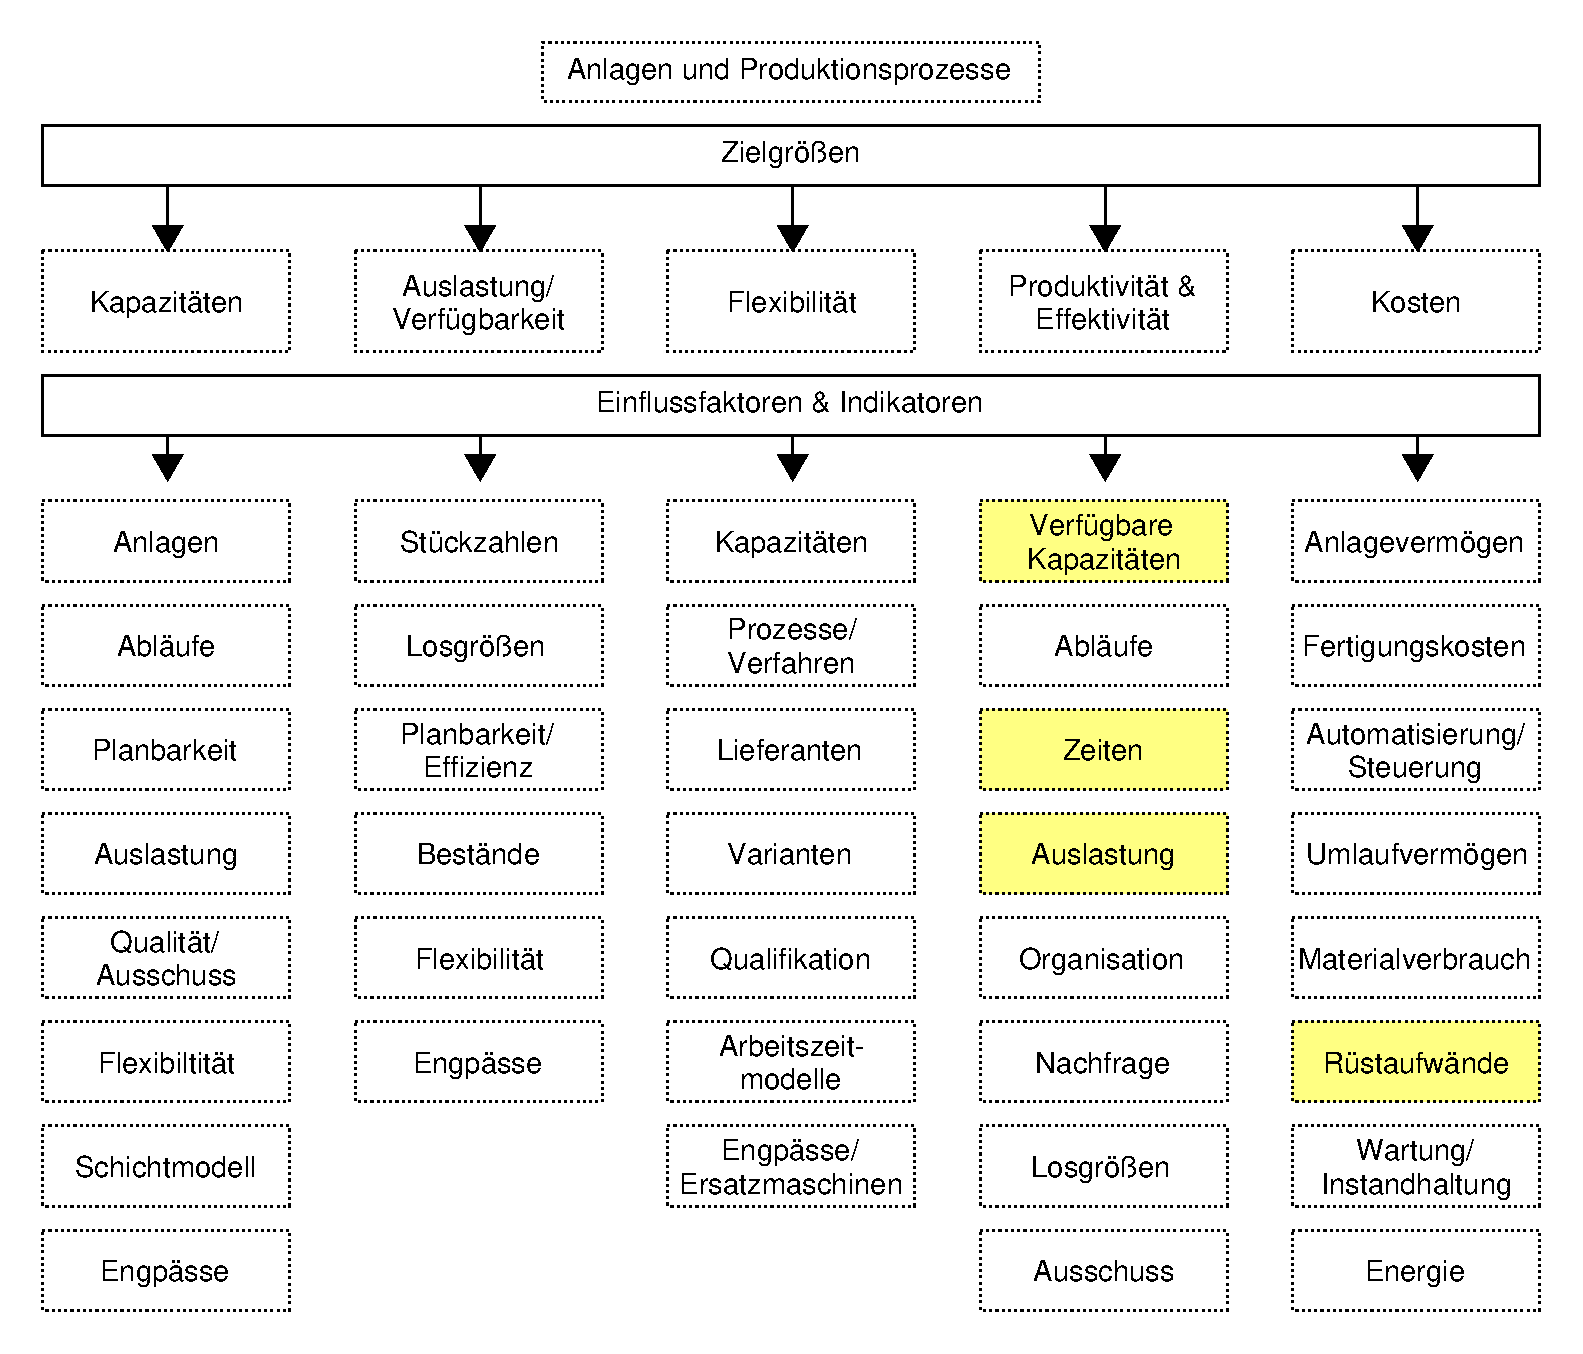
\includegraphics[scale=0.5]{DA_files/Bilder/Analyse/Produktionsprozesse-Zielgroessen.pdf}
\caption{x}
\label{pic:Produktionsprozesse-Zielgroessen}
\end{figure}

In dieser Arbeiten werden nur einige wenige Einflussfaktoren berücksichtigt. Zum einen ist nicht für jedes Unternehmen jede Zielgröße und somit auch nicht jeder Einflussfaktor relevant. Zum anderen ist beispielsweise die Flexibilität durch die modulare Anlage bereits weitestgehend gewährleistet. In dieser Arbeit wird der Fokus auf die Produktivität \& Effektivität und die Kosten gelegt. Die Produktivität beschreibt, wie viel der verfügbaren Arbeitszeit zur Produktion verwendet wird. Steht aufgrund vieler Störungen in der Anlage die Produktion still so ist die Produktivität gering. Bei einer hohen Effektivität werden die verfügbaren Ressourcen ideal genutzt. Dies kann beispielsweise die Zeit sein, die eine Reparatur in Anspruch nimmt. Die entstehenden Kosten sind für die Wirtschaftlichkeit der Produktion verantwortlich. Im Kontext des Modulaustausch sind vor allem die Anschaffungs- und Betriebskosten relevant. Folgende Einflussfaktoren sollen im weiteren Verlauf der Arbeit berücksichtigt werden:
\begin{itemize}
\item \textbf{Zeiten:} Wie viel Stillstandzeit verursacht der Modulaustausch?
\item \textbf{Auslastung:} Besteht die Möglichkeit vorzuproduzieren?
\item \textbf{Rüstaufwände:} Was muss alles im Rezept verändert werden? Welche Zeit nimmt das in Anspruch und welche Kosten verursacht das?
\item \textbf{Wartung:} Wie häufig muss das neue Modul gewartet werden?
\item \textbf{Energie:} Wie hoch ist der Energieverbrauch des Moduls? Welche Kosten verursacht dies beim Betrieb?
\end{itemize}

\section{Informationsanpassung}
Die Individualisierung von Software bietet die Möglichkeit eine Vielzahl von Nutzer und Aufgaben zu unterstützen. Individualisierung dient der Modifizierung von Interaktionen und Informationsdarstellungen, um den Fähigkeiten und Bedürfnissen jedes Benutzers gerecht zu werden. Zudem kann sich das System auch entsprechend der zu lösenden Aufgaben anpassen.

\subsection{Individualisierung für den Menschen}
Adaption.... Anpassung an

Jedes Unternehmen hat einen anderen Fokus. Andere Kennzahlen sind wichtig

\subsection{Anpassung an die Aufgabe}
Da die entstehenden Probleme sehr unterschiedlich sein können ist eine entsprechende Anpassung an die aktuelle Situation und die zu bearbeitende Aufgabe wichtig.

Wie schon in Abschnitt x beschrieben lassen sich Probleme anhand verschiedener Aspekte unterscheiden. So ist zum Beispiel der Zeitdruck ein wichtiger Aspekt. Bei zeitkritischen Problemen muss möglichst schnell eine gute Lösung gefunden werden. Ist das Problem nicht zeitkritisch so können in Ruhe alle zur Verfügung stehenden Informationen in den Problemlöseprozess mit einbezogen werden. So kann bei einem zeitkritischen Problem ein höherer Automatisierungsgrad gefordert sein. Um dennoch dem Menschen seine Kompetenzen nicht abzusprechen ist es möglich bei Problemen, die eher langfristig sind und die eine höhere kognitive Aktivität erfordern, eine geringere Autonomiestufe anzuwenden. Dadurch kann der Mensch sich Wissen über den Prozess aneignen und seine Kompetenzen ausbauen. 

Des weiteren unterscheidet sich maßgeblich, welche Informationen zur Verfügung gestellt werden müssen. Sendet ein Modul beispielsweise eine Warnung, dass der Füllstand den Grenzwert bald überschreitet so ist möglicherweise ein Hinweis notwendig, wie lange es noch dauert, bis der Behälter überläuft und was mögliche Konsequenzen sind.

\section{Interaktionsmechaniken}
Im Kontext dieser Arbeit wird das Problemlösen betrachtet. Problemlösen heißt in diesem Fall, dass beispielsweise die Ursache für eine Störung ausfindig gemacht werden muss. Die Behebung der Ursache, z.B. durch eine Reparatur, wird an dieser Stelle ausgeklammert. Im Stand der Technik sind verschiedene Interaktionsmechaniken beschrieben. Um diese geeignet bewerten zu können ist zunächst eine Begutachtung des Arbeitsumfelds und der Aufgaben notwendig. 

Welche Informationen muss der Nutzer eingeben können?? Welche Kriterien welche Priorität haben. 

\section{Anforderungen an das Assistenzsystem}

\subsection{Funktionale Anforderungen}

Unterstützung des Problemlöseprozess: Problem identifizieren. Ziel festlegen.

Probleme sortieren

Es muss eine Einschätzung erfolgen können, wie zeitkritisch das Problem ist

Es sollen mögliche Lösung miteinander verglichen werden können

Es muss der Zugang zum aktuellen Zustand der Anlage gewährleistet sein
-> Assistenzsystem markiert, was sich ändern würde

\subsection{Nichtfunktionale Anforderungen}

Das System soll auf einem Tablet ausgeführt werden
